\documentclass[11pt]{article}

\usepackage[margin=0.75in]{geometry}
\usepackage{amsmath,amssymb}
\usepackage{graphicx}
\usepackage{booktabs}
\usepackage{xcolor}
\usepackage[hidelinks]{hyperref}
\usepackage{titlesec}
\usepackage{float}
\usepackage{subcaption}

\titleformat{\section}{\large\bfseries}{\thesection}{1em}{}
\titleformat{\subsection}{\bfseries\color{blue!60!black}}{\thesubsection}{1em}{}
\titlespacing*{\section}{0pt}{10pt}{4pt}
\titlespacing*{\subsection}{0pt}{6pt}{3pt}
\setlength{\abovedisplayskip}{5pt}
\setlength{\belowdisplayskip}{5pt}
\captionsetup{font=small, skip=4pt}
\setlength{\intextsep}{6pt}

\title{\vspace{-0.5in}\Large\bfseries MSAI-635 Assignment 2: Gridworld and the Bellman Equations}
\author{Gaurav Prakash \\ UID: 122250130}
\date{\vspace{-0.35in}}

\begin{document}

\maketitle

\section{Problem Formulation}
\noindent\begin{minipage}[t]{0.6\textwidth}
\vspace{0pt}
The environment is a $4 \times 4$ gridworld. It is a finite Markov decision process (MDP) with 16 states numbered
row by row. $s_0$ (top-left) and $s_{15}$ (bottom-right) are terminal, and the other 14 are
non-terminal. In every non-terminal state the agent chooses one of four actions: up, down,
left, or right. The dynamics are deterministic: the agent moves one cell in the chosen
direction, and an action that would take it off the grid leaves it where it is (e.g.\ ``up''
from $s_2$ keeps the agent in $s_2$). Every transition yields reward $-1$, terminal states have
value $0$ and end the episode, and the discount factor is $\gamma = 1$.
\end{minipage}\hfill
\begin{minipage}[t]{0.37\textwidth}
\vspace{0pt}
\centering
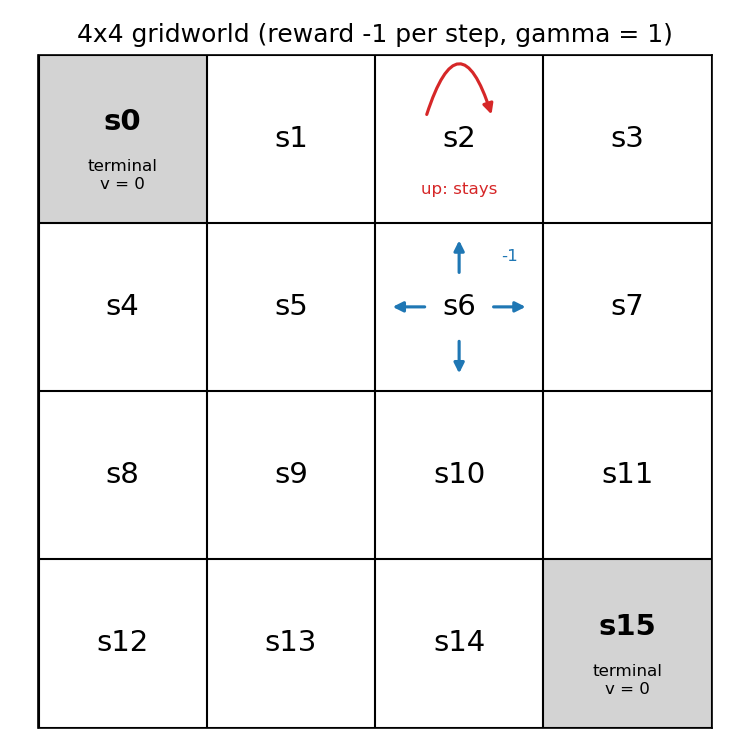
\includegraphics[width=\linewidth]{figures/gridworld_layout.png}
\captionof{figure}{4 * 4 gridworld. The red arrow shows the wall rule.}
\label{fig:grid}
\end{minipage}

\vspace{2pt}
Since every step costs $-1$ and nothing is discounted, the return of an episode is minus the
number of steps to reach a terminal, so a good policy reaches a corner quickly. The assignment has two goals:
(i) compute the state-value function $v_\pi$ of the \emph{uniform random policy},
$\pi(a \mid s) = 1/4$ for all states and actions, and
(ii) compute the \emph{optimal} value function $v_*$ and derive an optimal policy $\pi_*$ from it.

\section{Methodology}

\subsection{Bellman expectation equation (policy evaluation)}
The state value function under a policy $\pi$ is the total reward the agent can expect if it starts in
that state and keeps following the policy. The Bellman expectation equation says this
quantity can be computed one step at a time. A state is worth the reward of the next step plus
the discounted value of the state the agent lands in, \emph{averaged} over the actions the
policy might choose and the outcomes the environment might produce:
\[
v_\pi(s) = \sum_a \pi(a \mid s) \sum_{s', r} p(s', r \mid s, a)\,\bigl[r + \gamma\, v_\pi(s')\bigr].
\]
For the random policy every action has
weight $1/4$, so each value is the average of $-1 + v_\pi(s')$ over the four neighbors.
Writing the equation for each non-terminal state gives 14 linear equations in 14 unknowns.
\emph{Iterative policy evaluation} solves them by turning the equation into an update rule:
(1) initialize $V_0(s) = 0$; (2) sweep all non-terminal states, setting $V_{k+1}(s)$ to the
right-hand side evaluated with $V_k$ (terminal states stay at $0$); (3) stop when
$\Delta = \max_s |V_{k+1}(s) - V_k(s)| < \theta$. As a check, the same equations were also solved exactly as a linear system,
$(I - \gamma P_\pi)\,v = r_\pi$, where $P_\pi$ holds the transition probabilities between
non-terminal states under $\pi$ and $r_\pi$ the expected one-step rewards.

\subsection{Bellman optimality equation (value iteration)}
The Bellman optimality equation describes the value of acting \emph{as well as possible}
instead of following a fixed policy. The average over the policy's actions is replaced by a
\emph{maximum} over actions:
\[
v_*(s) = \max_a \sum_{s', r} p(s', r \mid s, a)\,\bigl[r + \gamma\, v_*(s')\bigr].
\]
This is the key difference from policy evaluation. Policy evaluation \emph{measures} a policy
that is given in advance: its equation is linear in $v$, and each policy has its own
solution. The optimality equation \emph{searches} over all policies at once through the max:
it is nonlinear, and its solution $v_*$ does not depend on any particular policy. \emph{Value iteration} applies the optimality equation as an
update, with the same initialization, sweeps and stopping rule as above. After convergence, an
optimal policy is obtained by acting greedily with respect to $v_*$,
$\pi_*(s) = \arg\max_a \sum_{s', r} p(s', r \mid s, a)\,[r + \gamma\, v_*(s')]$, keeping every action that ties for the maximum, since several moves can be equally good.

\subsection{Why the iterative updates converge}
Each sweep applies a Bellman operator $T$ (expectation or optimality) to the current estimate.
For $\gamma < 1$, both operators are $\gamma$-contractions in the max-norm,
$\|TV - TU\|_\infty \le \gamma\, \|V - U\|_\infty$. Every sweep therefore shrinks the distance to the true solution by at least a factor $\gamma$,
and by the Banach fixed-point theorem the iterates converge to the unique fixed point
($v_\pi$ or $v_*$) from any starting values. With $\gamma = 1$ this argument does not apply
directly, but convergence still holds because every episode reaches a terminal state with
probability 1. The matrix $P_\pi$ restricted to the non-terminal states ``leaks'' probability
into the terminals, so its spectral radius is below 1, and the error still shrinks
geometrically at rate $\rho(P_\pi)$. Intuitively, each sweep carries information from the terminals one step further across the grid.

\section{Experimental Setup}
\texttt{gridworld.py} defines the \texttt{GridWorld} class (grid layout, terminal and non-terminal states, transition dynamics,
next state and reward for any state--action pair); \texttt{policy\_evaluation.py} implements
iterative policy evaluation and the exact linear solve; \texttt{value\_iteration.py}
implements value iteration and greedy policy extraction; and \texttt{main.py} runs every
experiment and saves all figures.
Both algorithms start from $V_0 = 0$ and use $\gamma = 1$ and $\theta = 10^{-4}$. The main
results use the two-array (synchronous) update, in which every $V_{k+1}(s)$ is computed only
from $V_k$. An in-place variant (reusing values already updated in the same sweep) and runs varying the threshold
($\theta \in \{10^{-2}, \dots, 10^{-6}\}$) and the discount factor
($\gamma \in \{1, 0.9, 0.5, 0\}$) were added for comparison.

\section{Plots}
\begin{figure}[H]
\centering
\begin{subfigure}{0.32\textwidth}
  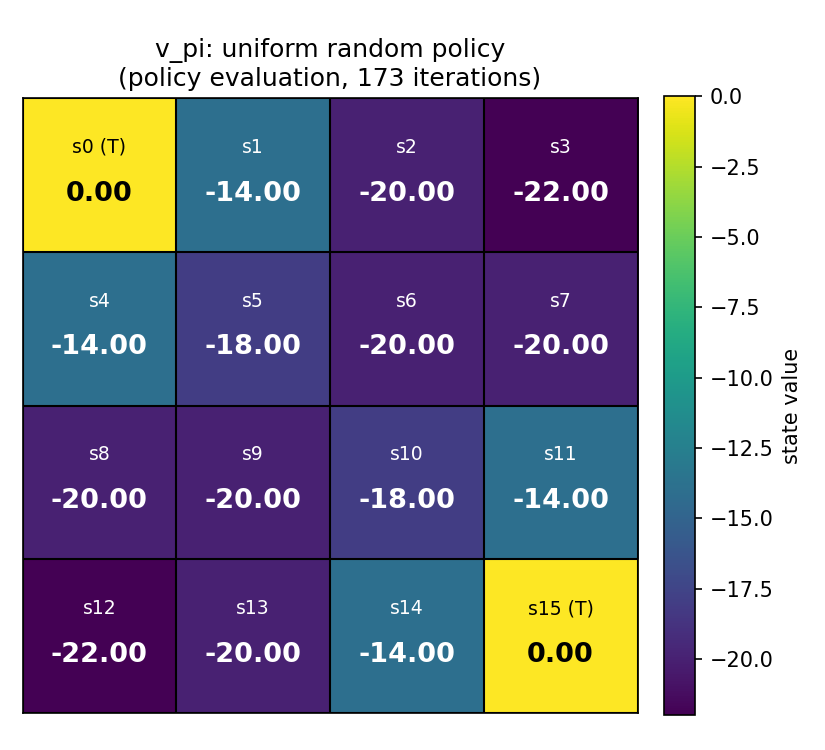
\includegraphics[width=\linewidth]{figures/policy_evaluation_values.png}
  \caption{$v_\pi$, random policy}
\end{subfigure}\hfill
\begin{subfigure}{0.32\textwidth}
  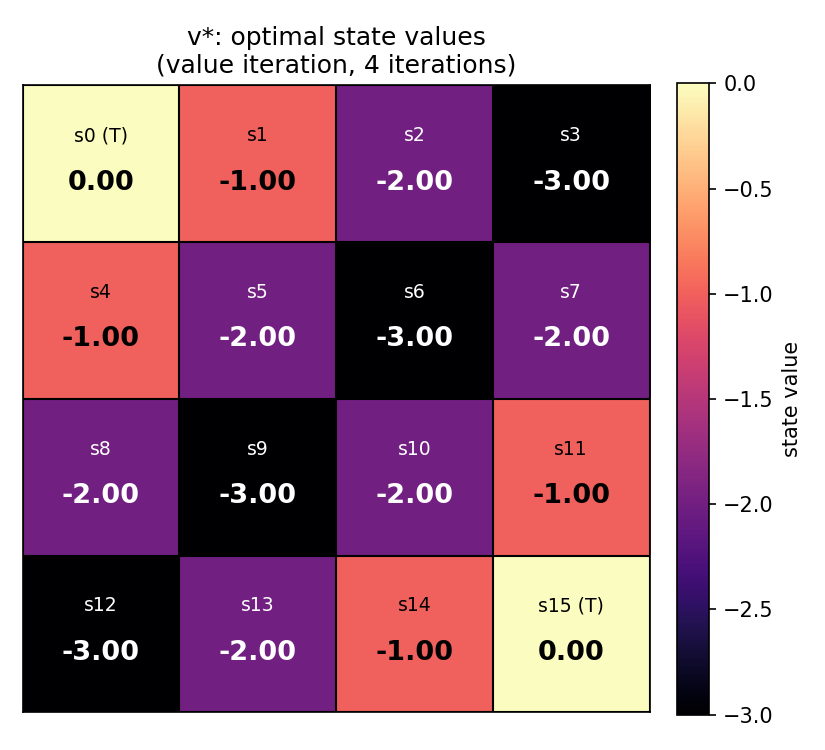
\includegraphics[width=\linewidth]{figures/optimal_values.png}
  \caption{$v_*$, value iteration}
\end{subfigure}\hfill
\begin{subfigure}{0.27\textwidth}
  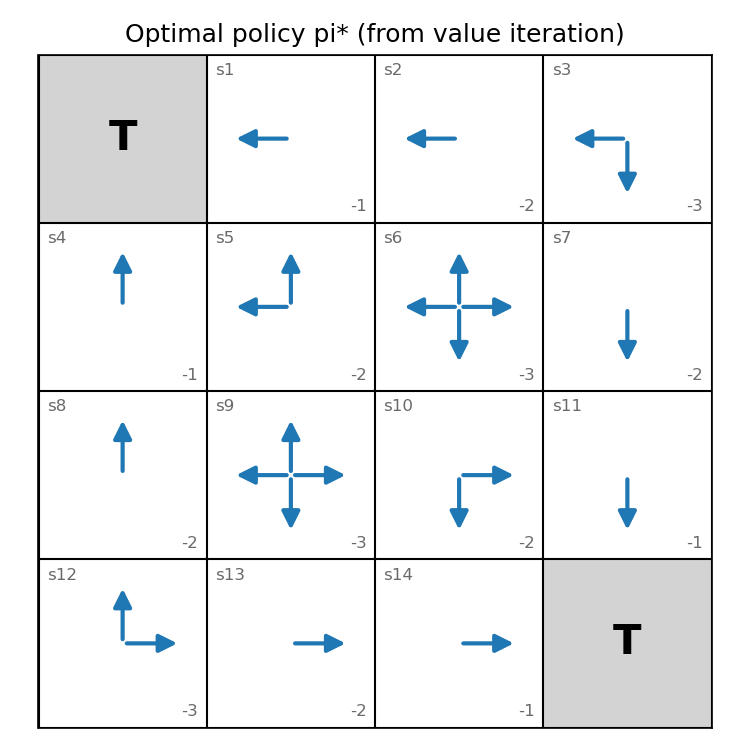
\includegraphics[width=\linewidth]{figures/optimal_policy.png}
  \caption{Optimal policy $\pi_*$}
\end{subfigure}
\caption{(a) State values under the uniform random policy after policy evaluation.
(b) Optimal state values after value iteration. (c) Greedy policy with respect to $v_*$:
several arrows in one cell are tied optimal actions, and T marks a terminal state.}
\label{fig:results}
\end{figure}

\section{Discussion}

\subsection{Random policy versus optimal value function}
Under the random policy (Figure~\ref{fig:results}a), values range from $-14$ next to the
terminals down to $-22$ in the far corners $s_3$ and $s_{12}$. With reward $-1$ per step and
$\gamma = 1$, $-v_\pi(s)$ is the \emph{expected number of steps} a random walk from $s$ takes
to reach a terminal state. The optimal values (Figure~\ref{fig:results}b) are
$v_*(s) = -d(s)$, where $d(s)$ is the shortest-path distance to the nearest terminal. Both
functions rank the states the same way: they are highest near the terminal corners and
symmetric about both diagonals. Their scale, however, is
very different: from $s_3$ a random agent needs 22 steps on average while an optimal agent
needs 3 (mean $-18.3$ vs.\ $-2.0$). The
gap $v_*(s) - v_\pi(s)$ measures the cost of acting randomly, since the random walk keeps
stepping away from the goal and bumping into walls. Even the greedy policy with respect to $v_\pi$ is
already optimal here (a subset of the tied actions in Figure~\ref{fig:results}c).

\subsection{Convergence speed}
Value iteration converges in 4 sweeps, while policy evaluation needs 173
(Figure~\ref{fig:convergence}). The difference comes from the max. Value iteration only follows
the shortest path, so after $k$ sweeps $V_k(s) = -\min(k, d(s))$; the values are exact after 3
sweeps, and the 4th sweep confirms convergence with $\Delta = 0$. Policy evaluation must account
for arbitrarily long random walks. In fact, $V_k(s) = -\mathbb{E}[\min(T, k)]$, where $T$ is
the number of steps to termination, so $\Delta_k$ is the probability that a walk from the worst
state is still going after $k - 1$ steps. This probability decays geometrically at rate
$\rho(P_\pi) \approx 0.947$: a walk that has not ended has only
about a 5\% chance of ending on the next step. Solving $\Delta_k \approx 1.26\,\rho^k < 10^{-4}$
gives $k \approx 173$. The same rate explains why each $10\times$ smaller $\theta$ adds about
$\ln 10 / \ln(1/\rho) \approx 42$ sweeps (Table~\ref{tab:theta}), and why the final error
($1.8 \times 10^{-3}$) is larger than $\theta$: the remaining sweeps would still add about
$\Delta\, \rho / (1 - \rho)$. The in-place variant needs only 114 sweeps because values updated early in a sweep are reused immediately.

\subsection{Effect of the discount factor}
Lowering $\gamma$ makes all values less
negative, because costs far in the future are shrunk: for the optimal policy,
$v_*(s) = -(1 - \gamma^{d(s)})/(1 - \gamma)$ instead of $-d(s)$. The random policy is affected
much more, because its paths are long ($v_\pi(s_3)$ goes from $-22$ to $-7.65$ at
$\gamma = 0.9$; Table~\ref{tab:gamma}). Convergence also speeds up, since the error now shrinks
at rate $\gamma\rho$ instead of $\rho$ (173 $\to$ 60 $\to$ 14 sweeps). The optimal policy stays
the same for every $\gamma \in (0, 1]$: all rewards are equal and negative, so reaching a
terminal sooner is always better and the shortest path remains optimal. At $\gamma = 0$ the
agent is completely myopic. Every action costs exactly $-1$ and the future is ignored, so all
actions tie and the policy no longer points toward the goal. In problems with mixed rewards
(for example, a large distant reward against a small nearby one), changing $\gamma$ can change
the optimal policy itself, not just the values.

\section{Results}
At the main setting ($\gamma = 1$, $\theta = 10^{-4}$),
policy evaluation takes 173 sweeps (114 in-place) and ends within $1.8 \times 10^{-3}$ of the exact
solution, while value iteration is exact after 4 sweeps (Figure~\ref{fig:convergence}).
Tables~\ref{tab:theta} and~\ref{tab:gamma} vary $\theta$ and $\gamma$.

\noindent\begin{minipage}[c]{0.47\textwidth}
\centering
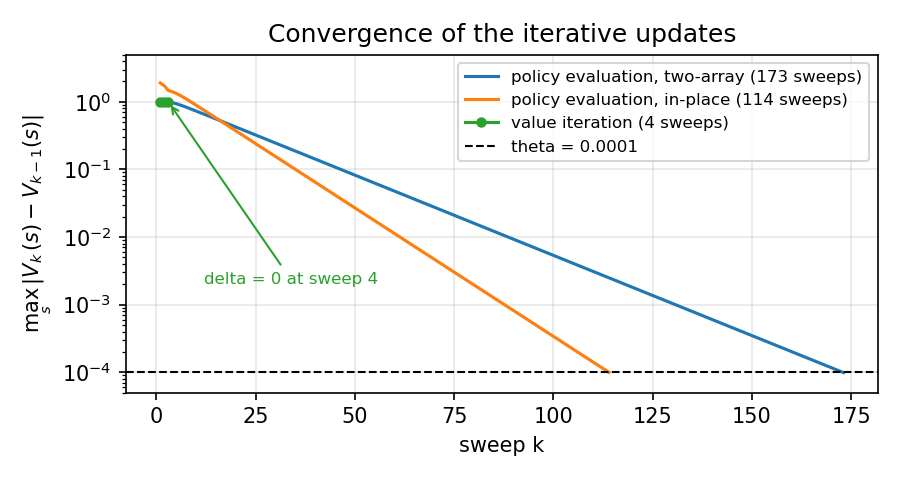
\includegraphics[width=\linewidth]{figures/convergence.png}
\captionof{figure}{Largest change per sweep (log scale).}
\label{fig:convergence}
\end{minipage}\hfill
\begin{minipage}[c]{0.5\textwidth}
\centering
\small
\begin{tabular}{ccccc}
\toprule
$\theta$ & \multicolumn{2}{c}{two-array} & \multicolumn{2}{c}{in-place} \\
         & iters & error & iters & error \\
\midrule
$10^{-2}$ & 89  & $1.7\mathrm{e}{-1}$ & 62  & $1.0\mathrm{e}{-1}$ \\
$10^{-3}$ & 131 & $1.7\mathrm{e}{-2}$ & 88  & $1.1\mathrm{e}{-2}$ \\
$10^{-4}$ & 173 & $1.8\mathrm{e}{-3}$ & 114 & $1.1\mathrm{e}{-3}$ \\
$10^{-5}$ & 215 & $1.8\mathrm{e}{-4}$ & 141 & $1.0\mathrm{e}{-4}$ \\
$10^{-6}$ & 258 & $1.7\mathrm{e}{-5}$ & 167 & $1.1\mathrm{e}{-5}$ \\
\bottomrule
\end{tabular}
\captionof{table}{Policy evaluation ($\gamma = 1$) vs.\ threshold $\theta$; error is the max
deviation from the exact linear solution.}
\label{tab:theta}
\end{minipage}

\begin{table}[H]
\centering
\small
\begin{tabular}{cccccc}
\toprule
$\gamma$ & PE iters & $v_\pi(s_3)$ & VI iters & $v_*(s_3)$ & $\pi_*$ \\
\midrule
1.0 & 173 & $-22.00$ & 4 & $-3.00$ & shortest path \\
0.9 & 60  & $-7.65$  & 4 & $-2.71$ & shortest path \\
0.5 & 14  & $-1.98$  & 4 & $-1.75$ & shortest path \\
0.0 & 2   & $-1.00$  & 2 & $-1.00$ & all actions tie \\
\bottomrule
\end{tabular}
\caption{Effect of $\gamma$ ($\theta = 10^{-4}$; PE = policy evaluation, VI = value iteration).}
\label{tab:gamma}
\end{table}

\section{Conclusions}
Iterative policy evaluation recovered the random policy's value function ($-14$ to $-22$) in
173 iterations, matching the exact linear solution, while value iteration found
$v_*(s) = -d(s)$ in 4 iterations, with a greedy policy that follows shortest paths to the
terminals. The expectation equation measures a fixed behavior, while the optimality equation
finds the best one. Both converge because each Bellman sweep shrinks the error, and the rate of
that shrinking explains the gap in iteration counts. The discount factor changes the scale of
the values and the speed of convergence, but here it leaves the optimal policy unchanged for
every $\gamma > 0$.

\end{document}
